


The rise of large language models (LLMs) as a general-purpose tool for a diverse range of natural language processing tasks has dramatically transformed the field, introducing new paradigms for data collection and model training 
(\citealp{brown2020language}, \citealp{biderman2023pythia}, \citealp{touvron2023llama}, 
\citealp{jiang2023mistral}, 
\citealp{chowdhery2023palm}, \citealp{groeneveld2024olmo}, \citealp{wang2024helpsteer2}, \textit{inter alia}).
Numerous models, training methods, datasets, and evaluation methods continue to be developed on an ongoing basis.
Nevertheless, a unified paradigm has emerged for training LLMs: pre-train on an enormous corpus of diverse documents, ranging from 250B \cite{biderman2023pythia} to 15T \cite{llama3modelcard} tokens, followed by an alignment stage to make the model more useful and performative for various tasks.

\twocolumn[{%
	\renewcommand\twocolumn[1][]{#1}%
	\maketitle
	\begin{center}
		\newcommand{\teaserwidth}{\textwidth}
		% \vspace{-0.15in}
		\centerline{
			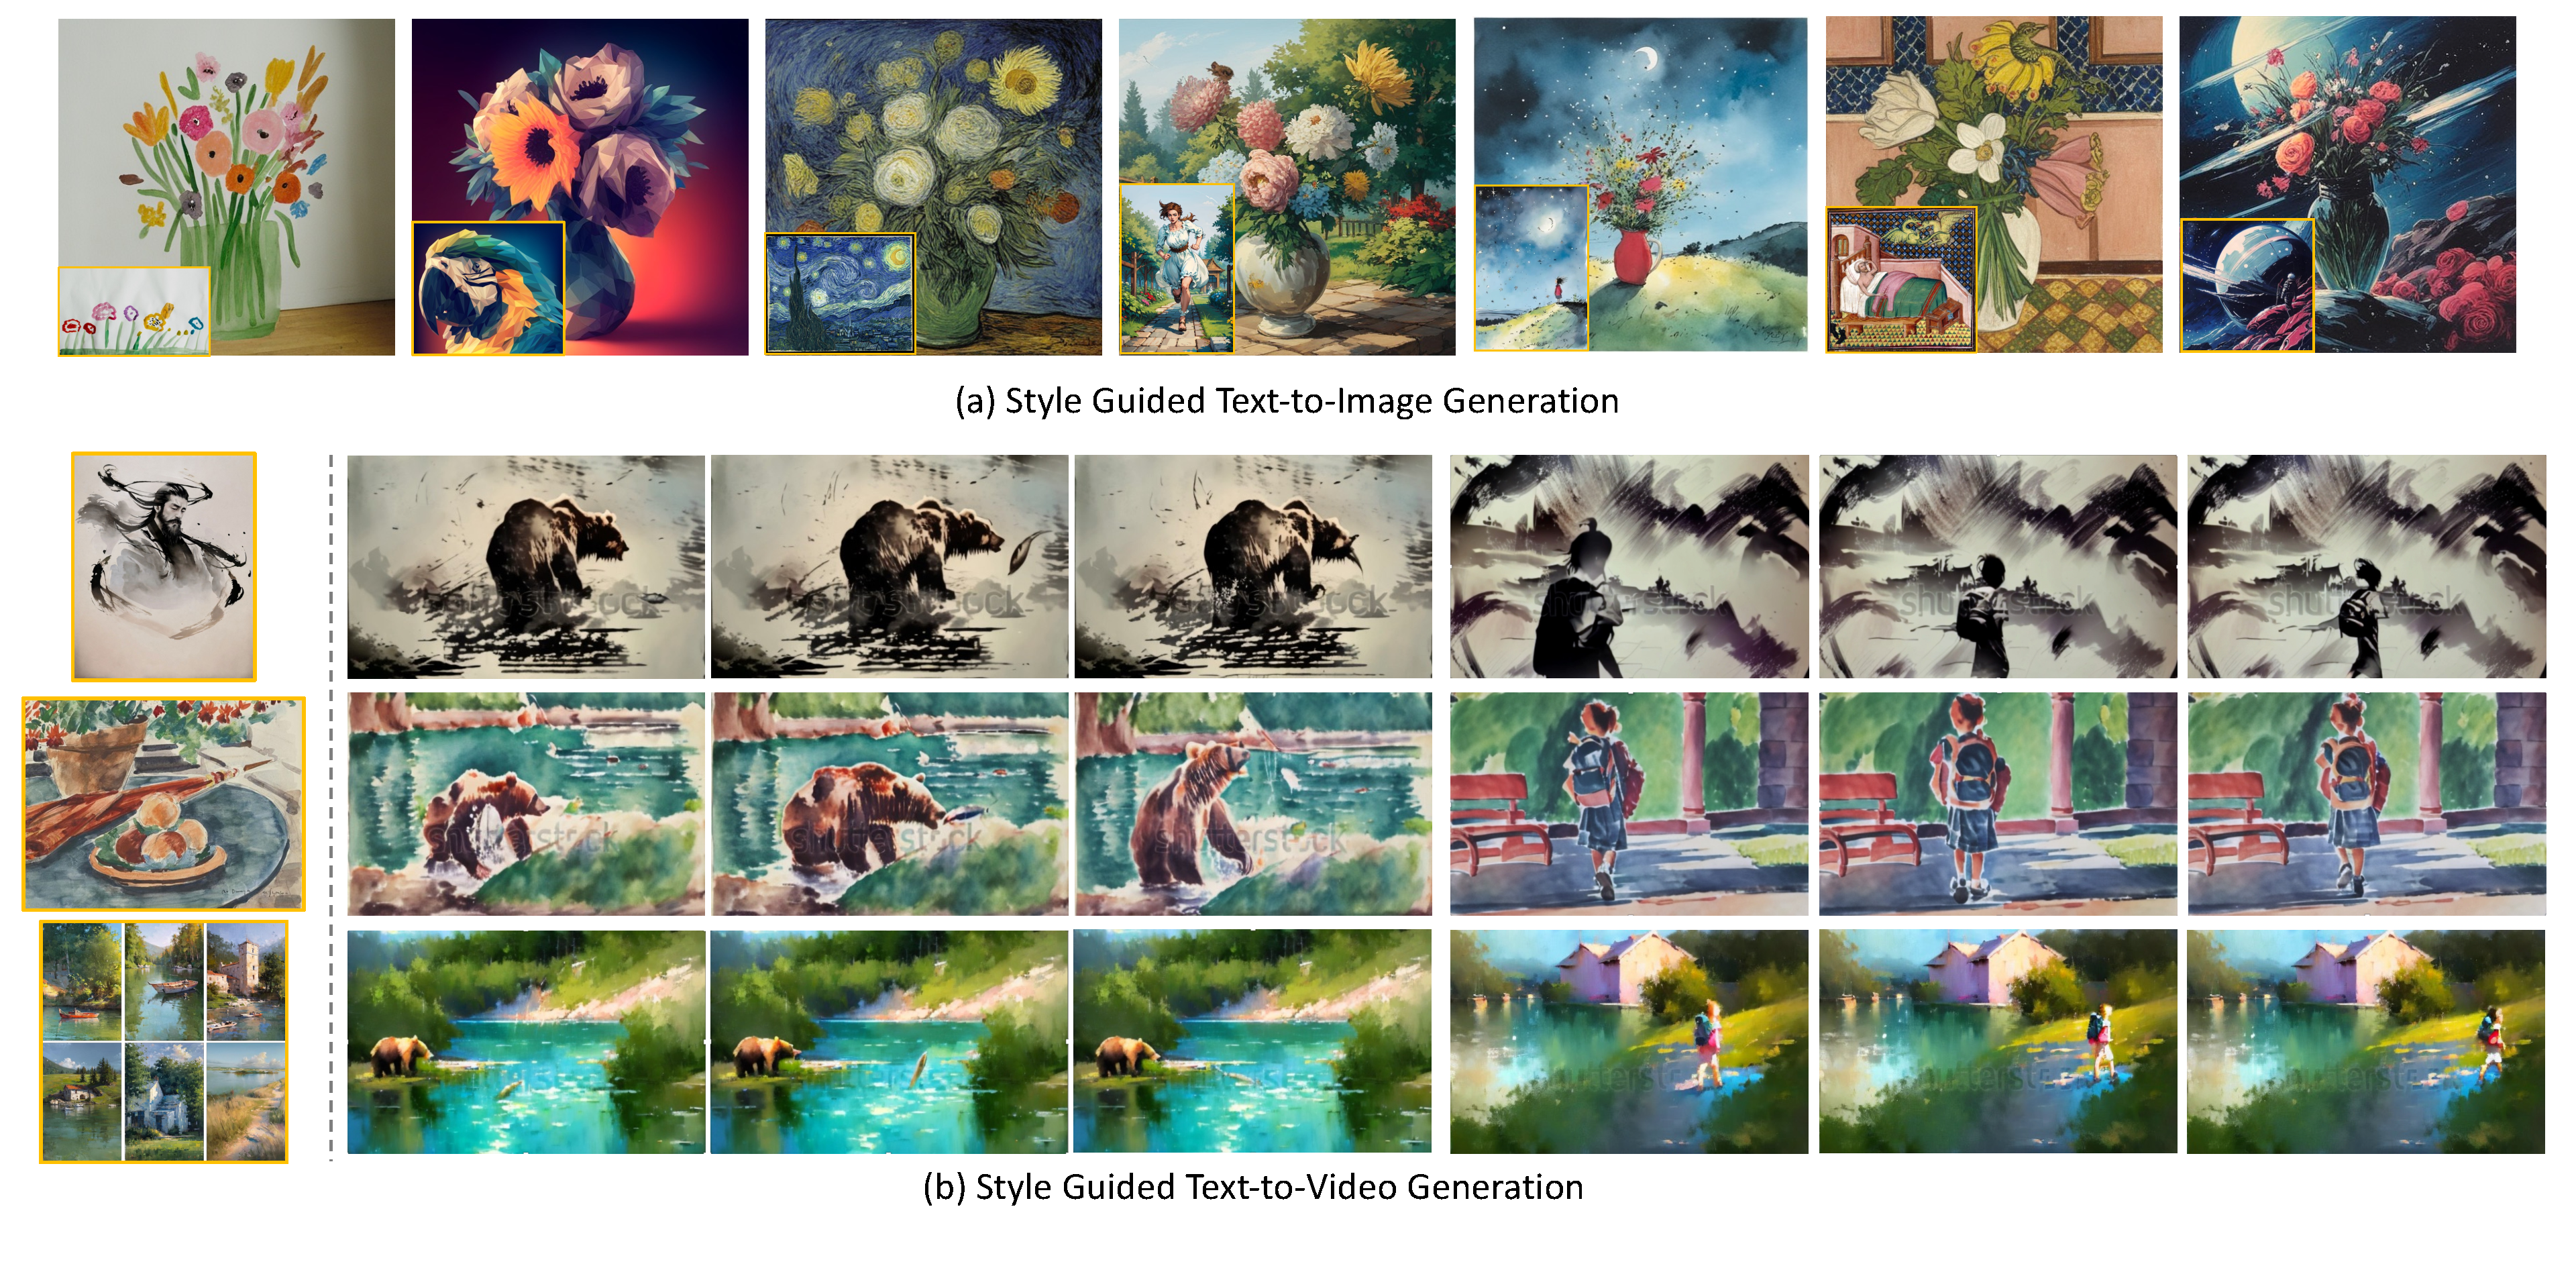
\includegraphics[width=\teaserwidth,clip]{figures/pdf_files/teaser.pdf}
		}
		\vspace{-1ex}
		\captionof{figure}{\textbf{Human Gaussian Splats (\acronym)} is a neural rendering framework that trains on 50-100 frames of a monocular video containing a human in a scene. HUGS enables novel view rendering with novel human poses at 60 FPS by learning a disentangled representation that can also render the human in other scenes. }
		% \vspace{-0.08in}
		\label{fig:teaser}
	\end{center}%
}]
Based on this paradigm, work has focused on improving these two stages. 
Work to improve pre-trained models includes larger training sets \cite{hoffmann2022training, llama3modelcard, touvron2023llama}, different data selection mechanisms \cite{xia2024less}, higher quality data \cite{zhou2024lima}, and various model architectures \cite{su2024roformer, touvron2023llama}. 
Meanwhile, research on model alignment includes different training objectives \cite{rafailov2024direct, schulman2017proximal},
new datasets \cite{narayanan-aepli-2024-tulu-resource}, more efficient training \cite{hu2021lora,dettmers2024qlora} and safety tuning \cite{bianchi2023safety}. The alignment stage usually involves either supervised fine-tuning for specific tasks or instruction fine-tuning for general-purpose usage. 
Regardless, fine-tuning (almost always) comes at the end of pre-training and yields remarkable improvements on downstream tasks \cite{touvron2023llama, groeneveld2024olmo}. 
Consequently, the benefits of each stage are largely explored independently, with improvements to pretraining being orthogonal to benefits from model alignment.

Rather than explore these two training regimes independently, we question: {\bf how do model pretraining and fine-tuning interact to affect the resulting model?} Does more pre-training hinder better fine-tuning results? What does the model learn and forget during pre-training as well as fine-tuning?
Answering these questions requires us to examine how models learn during pre-training and how this affects fine-tuning. Therefore, 
we fine-tune {\bf multiple pre-training checkpoints} of a large language model (Figure~\ref{fig:experiment-illu}), evaluating each checkpoint and its fine-tuned version on downstream evaluation sets.
We track model abilities during pre-training and compare them to improvements achievable after fine-tuning at the corresponding pre-training step.
We explore both supervised and instruction fine-tuning, testing the models' memorization and forgetting when learning specific tasks and serving as general-purpose language-AI tools. 
To the best of our knowledge, we are the first to explore fine-tuning intermediate model checkpoints.

Our experiments yield insights into LLM training.
We find that (1) continued pre-training can improve a model in ways that are only revealed after fine-tuning (\sect{sec:finding:PTFT}); (2) tasks for which the model already performs well during pre-training benefit much less from fine-tuning than those where the model does not demonstrate capabilities (\sect{sec:finding:base-eval}, \sect{sec:finding:PTFT}); (3) although supervised fine-tuning can improve performance on in-distribution tasks, it can also cause the model to forget domain knowledge or tasks that it was previously capable of solving (\sect{sec:finding:what}); (4) fine-tuned models show high sensitivity to evaluation prompts, but this sensitivity can be alleviated by more pre-training (\sect{sec:finding:what}).
Our findings provide insights into model training and can inform methods for both pre-training and fine-tuning. Furthermore, our work shows the value of analyzing the training dynamics, in addition to analyzing the final LLM, as an aspect of interpretability, and we encourage model developers to release these checkpoints to aid future studies.
